\section{Converter setup}
\label{sec:setup}

\subsection{Ozone generator setup}
\label{sec:ozone-setup}

As a proof of concept we built the Ozone generator on a wooden board
as can be seen in Figure~\ref{fig:setup}. As described in
Section~\ref{sec:requirements}, the lab air was first filtered and
then sent through an alluminium coated tube containting a Pen-Ray
Hg-Lamp (Model 11SC-1). It has a lighted length of
\SI{53.8}{\milli\meter} and primary energy at
\SI{254}{\nano\meter}. The primary energy setting is not perfect for
our purposes as it is directly at the Ozone dissociation wavelength,
where as the lamp has almost no energy output at the Oxygen
dissociation wavelength. However, since the Oxygen concentration in
ambient air is so high, we would still expect enough Ozone to be
produced. 
To make sure the superfluous \ch{NO} is completely converted to
\ch{NO2}, we introduce a \SI{3}{\meter} teflon tube. Afterwards the
Ozone enriched air passed another Silica gel filter and is expected to
then be \ch{NO_x} free.

To be able to measure the Ozone production after the last filter a
cuvette was added, which could be entered in the light path of a
longpath DOAS instrument (cf.\ Fig.~\ref{fig:cuvette}). The length of
the lightpath through the cuvette is \SI{10}{\centi\meter}. 

The Pen-Ray power source could switch the current between
\SI{10}{\milli\ampere} and \SI{17}{\milli\ampere}.  Furthermore the
Flow $\Phi_{\ch{O 3}}$ could be set via the flowmeter between \num{0}
and \SI{0.3}{\liter\per\minute}. The lowest stable flow higher than
\SI{0}{\liter\per\minute} was \SI{0.03}{\liter\per\minute}.

\begin{figure}[htbp]
  \centering
  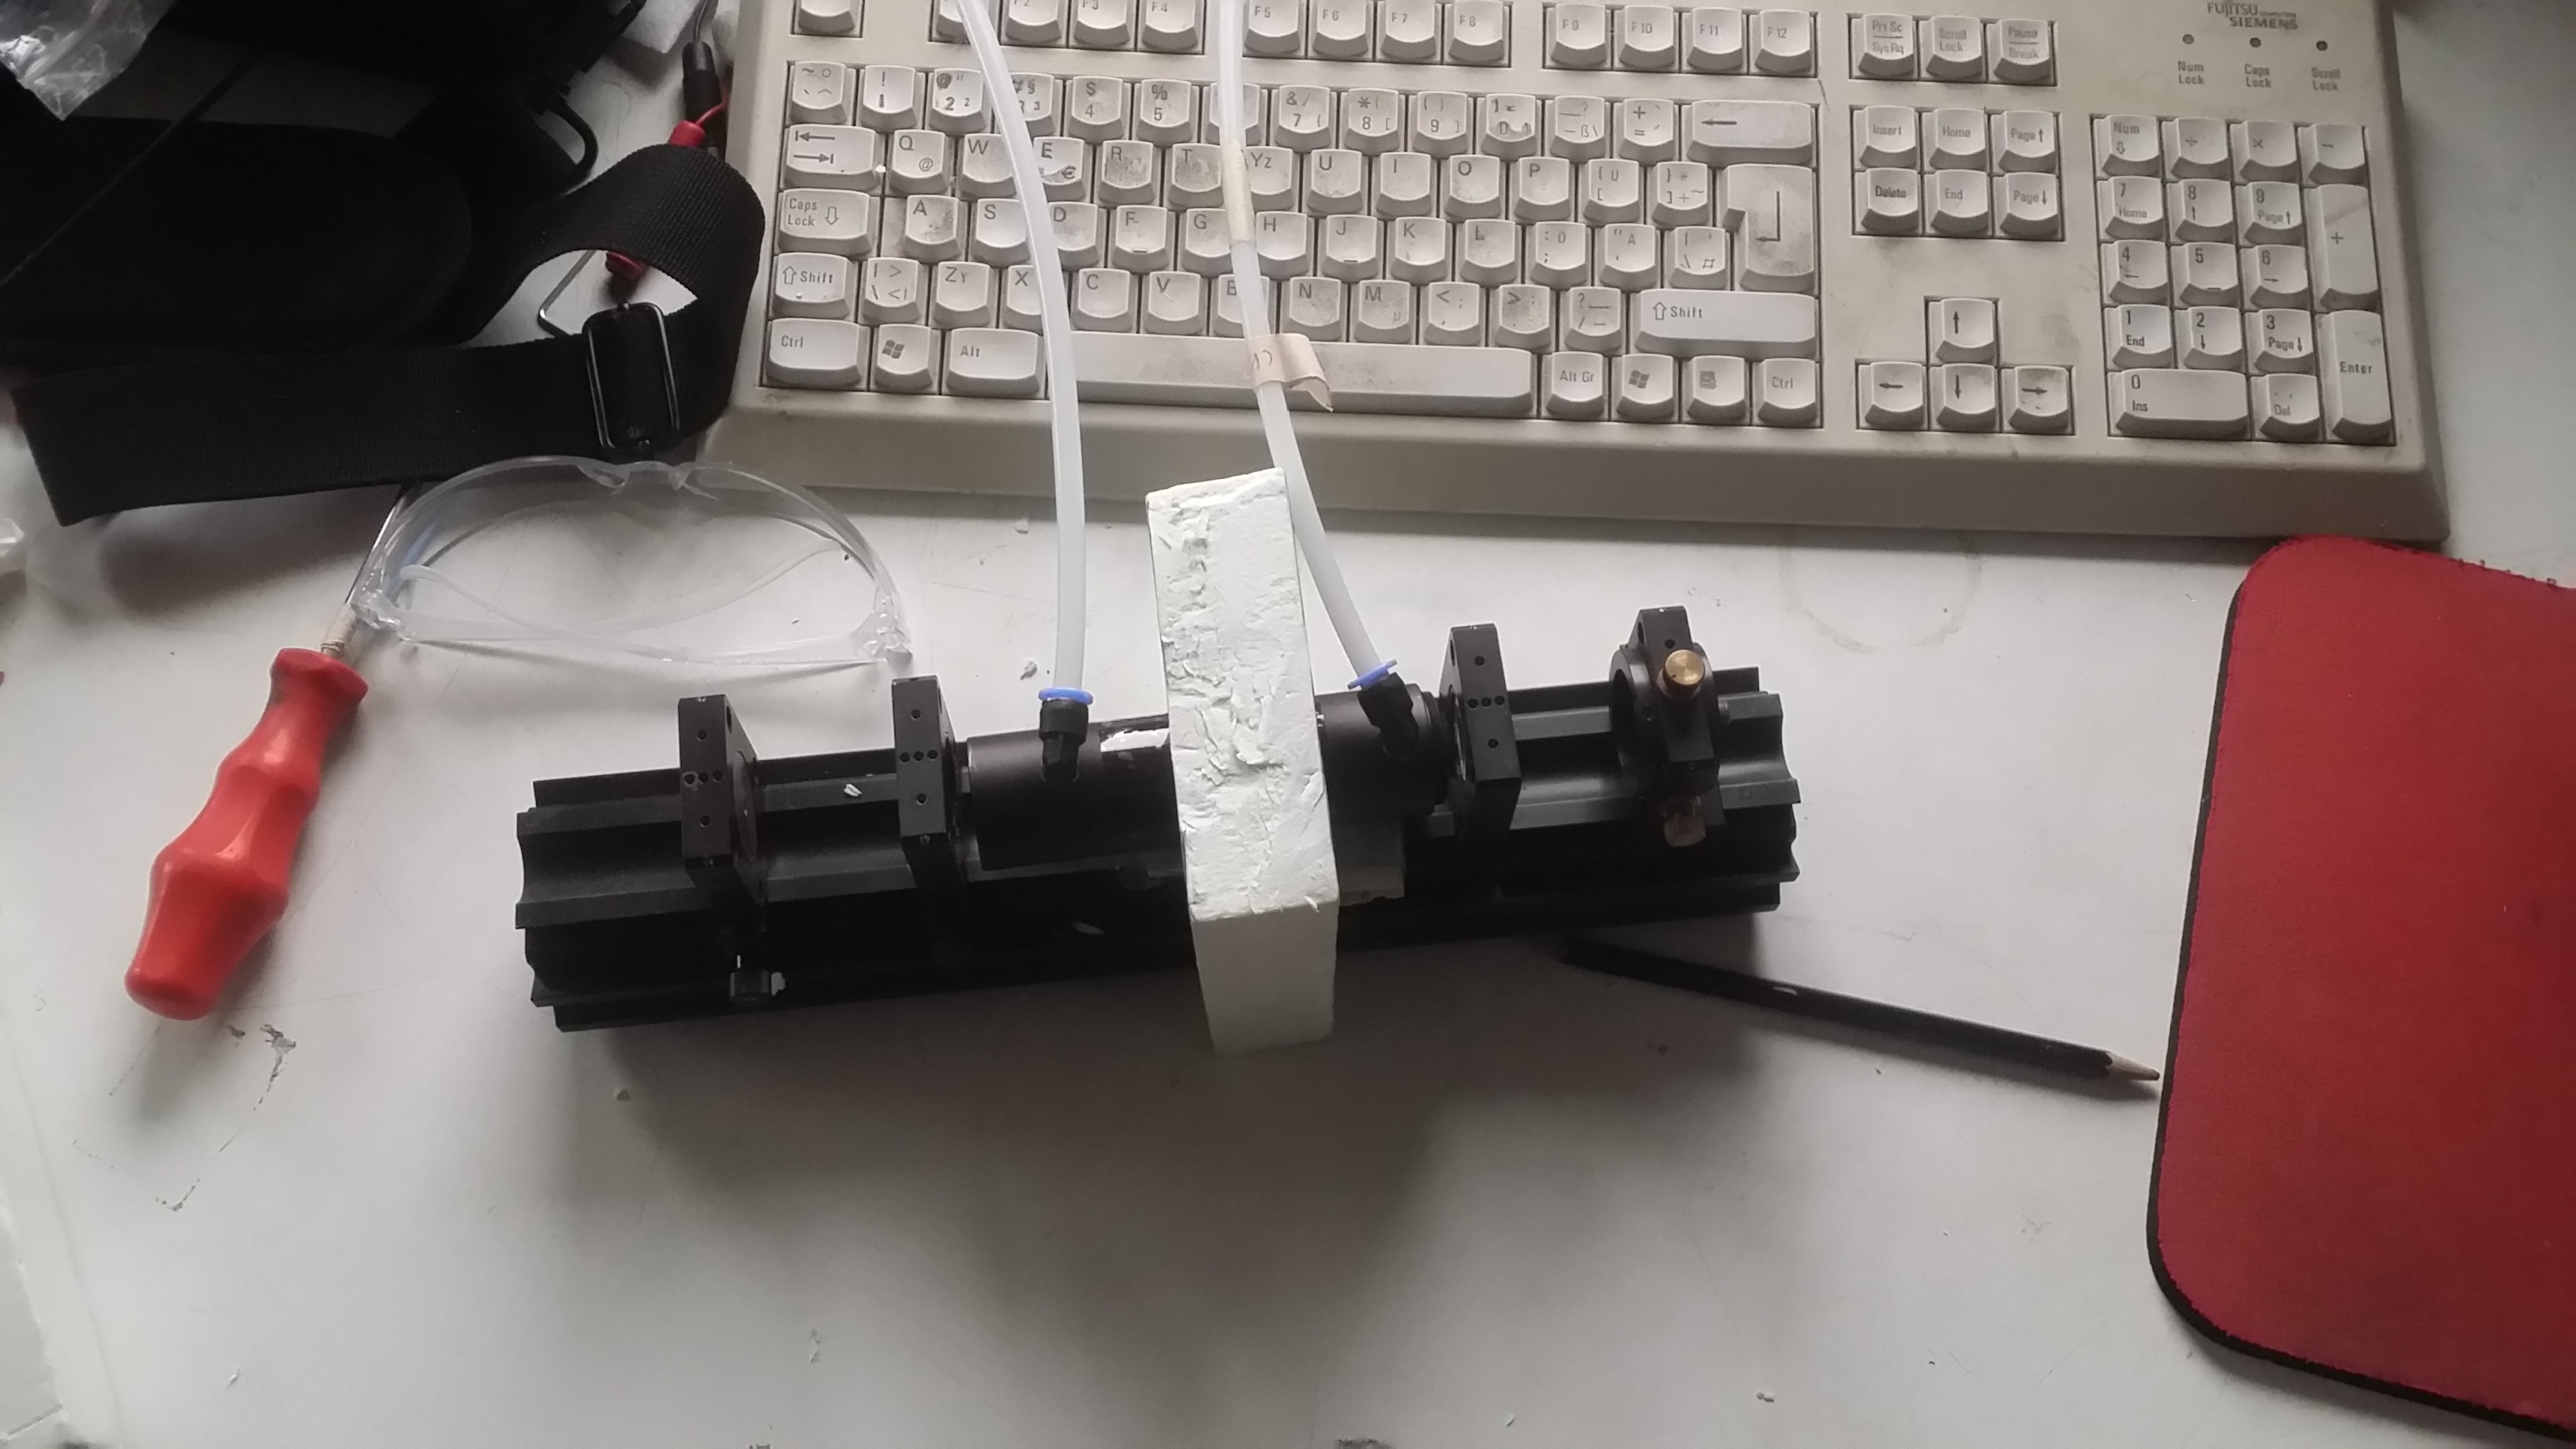
\includegraphics[width=0.7\textwidth]{images/cuvette.jpg}
  \caption{Cuvette together with styrofoam mount on an optical
    rack. The outermost riders are the mounts for the optical
    fibers. The riders within consist of two collimators.}
  \label{fig:cuvette}
\end{figure}

\begin{figure}[htbp]
  \centering
  {
  \def\svgwidth{0.9\linewidth}
  %% Creator: Inkscape inkscape 0.91, www.inkscape.org
%% PDF/EPS/PS + LaTeX output extension by Johan Engelen, 2010
%% Accompanies image file 'setup.pdf_tex.pdf' (pdf, eps, ps)
%%
%% To include the image in your LaTeX document, write
%%   \input{<filename>.pdf_tex}
%%  instead of
%%   \includegraphics{<filename>.pdf}
%% To scale the image, write
%%   \def\svgwidth{<desired width>}
%%   \input{<filename>.pdf_tex}
%%  instead of
%%   \includegraphics[width=<desired width>]{<filename>.pdf}
%%
%% Images with a different path to the parent latex file can
%% be accessed with the `import' package (which may need to be
%% installed) using
%%   \usepackage{import}
%% in the preamble, and then including the image with
%%   \import{<path to file>}{<filename>.pdf_tex}
%% Alternatively, one can specify
%%   \graphicspath{{<path to file>/}}
%% 
%% For more information, please see info/svg-inkscape on CTAN:
%%   http://tug.ctan.org/tex-archive/info/svg-inkscape
%%
\begingroup%
  \makeatletter%
  \providecommand\color[2][]{%
    \errmessage{(Inkscape) Color is used for the text in Inkscape, but the package 'color.sty' is not loaded}%
    \renewcommand\color[2][]{}%
  }%
  \providecommand\transparent[1]{%
    \errmessage{(Inkscape) Transparency is used (non-zero) for the text in Inkscape, but the package 'transparent.sty' is not loaded}%
    \renewcommand\transparent[1]{}%
  }%
  \providecommand\rotatebox[2]{#2}%
  \ifx\svgwidth\undefined%
    \setlength{\unitlength}{1567.76523438bp}%
    \ifx\svgscale\undefined%
      \relax%
    \else%
      \setlength{\unitlength}{\unitlength * \real{\svgscale}}%
    \fi%
  \else%
    \setlength{\unitlength}{\svgwidth}%
  \fi%
  \global\let\svgwidth\undefined%
  \global\let\svgscale\undefined%
  \makeatother%
  \begin{picture}(1,0.56250002)%
    \put(0,0){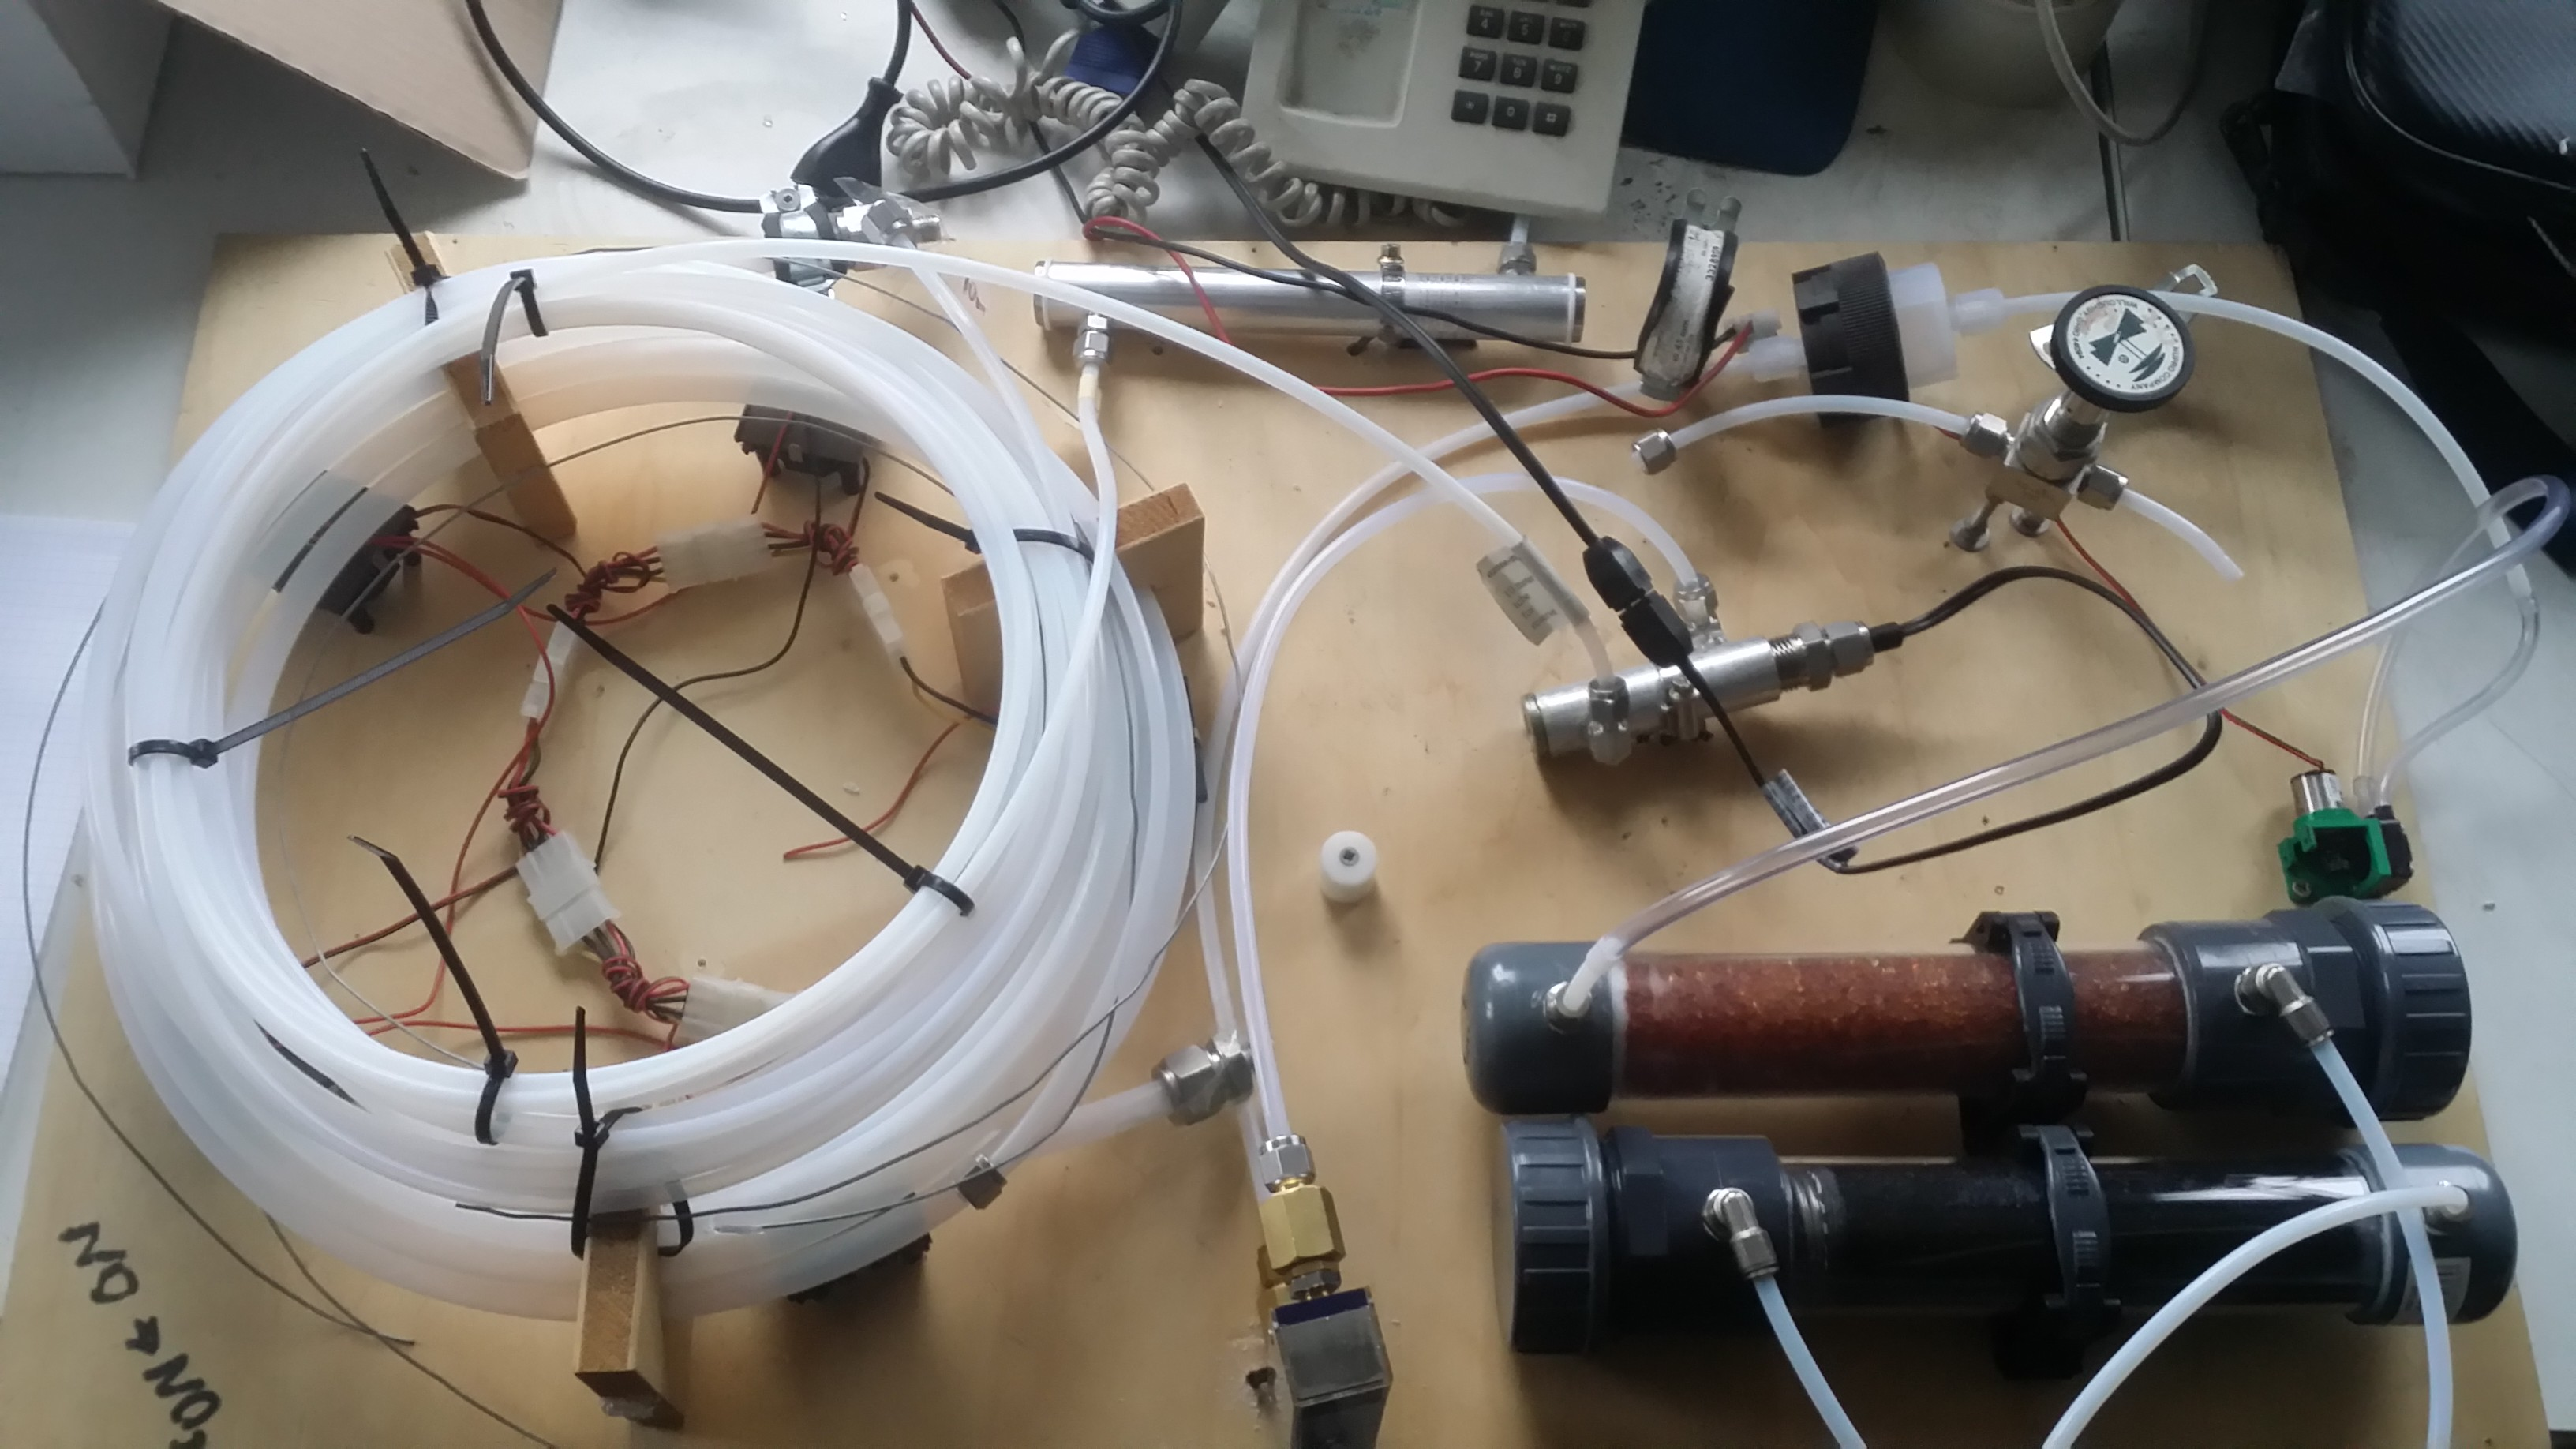
\includegraphics[width=\unitlength,page=1]{setup.pdf}}%
    \put(0.72339254,0.0272422){\color[rgb]{0,0,0}\makebox(0,0)[lb]{carbon filter}}%
    \put(0.68467052,0.20608212){\color[rgb]{0,0,0}\makebox(0,0)[lb]{\smash{silica gel}}}%
    \put(0.84485225,0.27636329){\color[rgb]{0,0,0}\makebox(0,0)[lb]{\smash{pump}}}%
    \put(0.66524548,0.47215208){\color[rgb]{0,0,0}\makebox(0,0)[lb]{\smash{particle filter}}}%
    \put(0.37854499,0.02340413){\color[rgb]{0,0,0}\makebox(0,0)[lb]{\smash{flowmeter}}}%
    \put(0.41093385,0.46876799){\color[rgb]{0,0,0}\makebox(0,0)[lb]{\smash{silica gel in tube}}}%
    \put(0.55474278,0.26558162){\color[rgb]{0,0,0}\makebox(0,0)[lb]{\smash{penray lamp in tube}}}%
    \put(0,0){\includegraphics[width=\unitlength,page=2]{setup.pdf}}%
    \put(1.00286136,0.04729665){\color[rgb]{0,0,0}\makebox(0,0)[lb]{\smash{lab air}}}%
    \put(0.59985726,0.5399915){\color[rgb]{0,0,0}\makebox(0,0)[lb]{\smash{ozone}}}%
    \put(0,0){\includegraphics[width=\unitlength,page=3]{setup.pdf}}%
  \end{picture}%
\endgroup%

%%% Local Variables:
%%% mode: latex
%%% TeX-master: "../Bachelor"
%%% End:

  }
  \phantom{h}\\
  \bigskip
  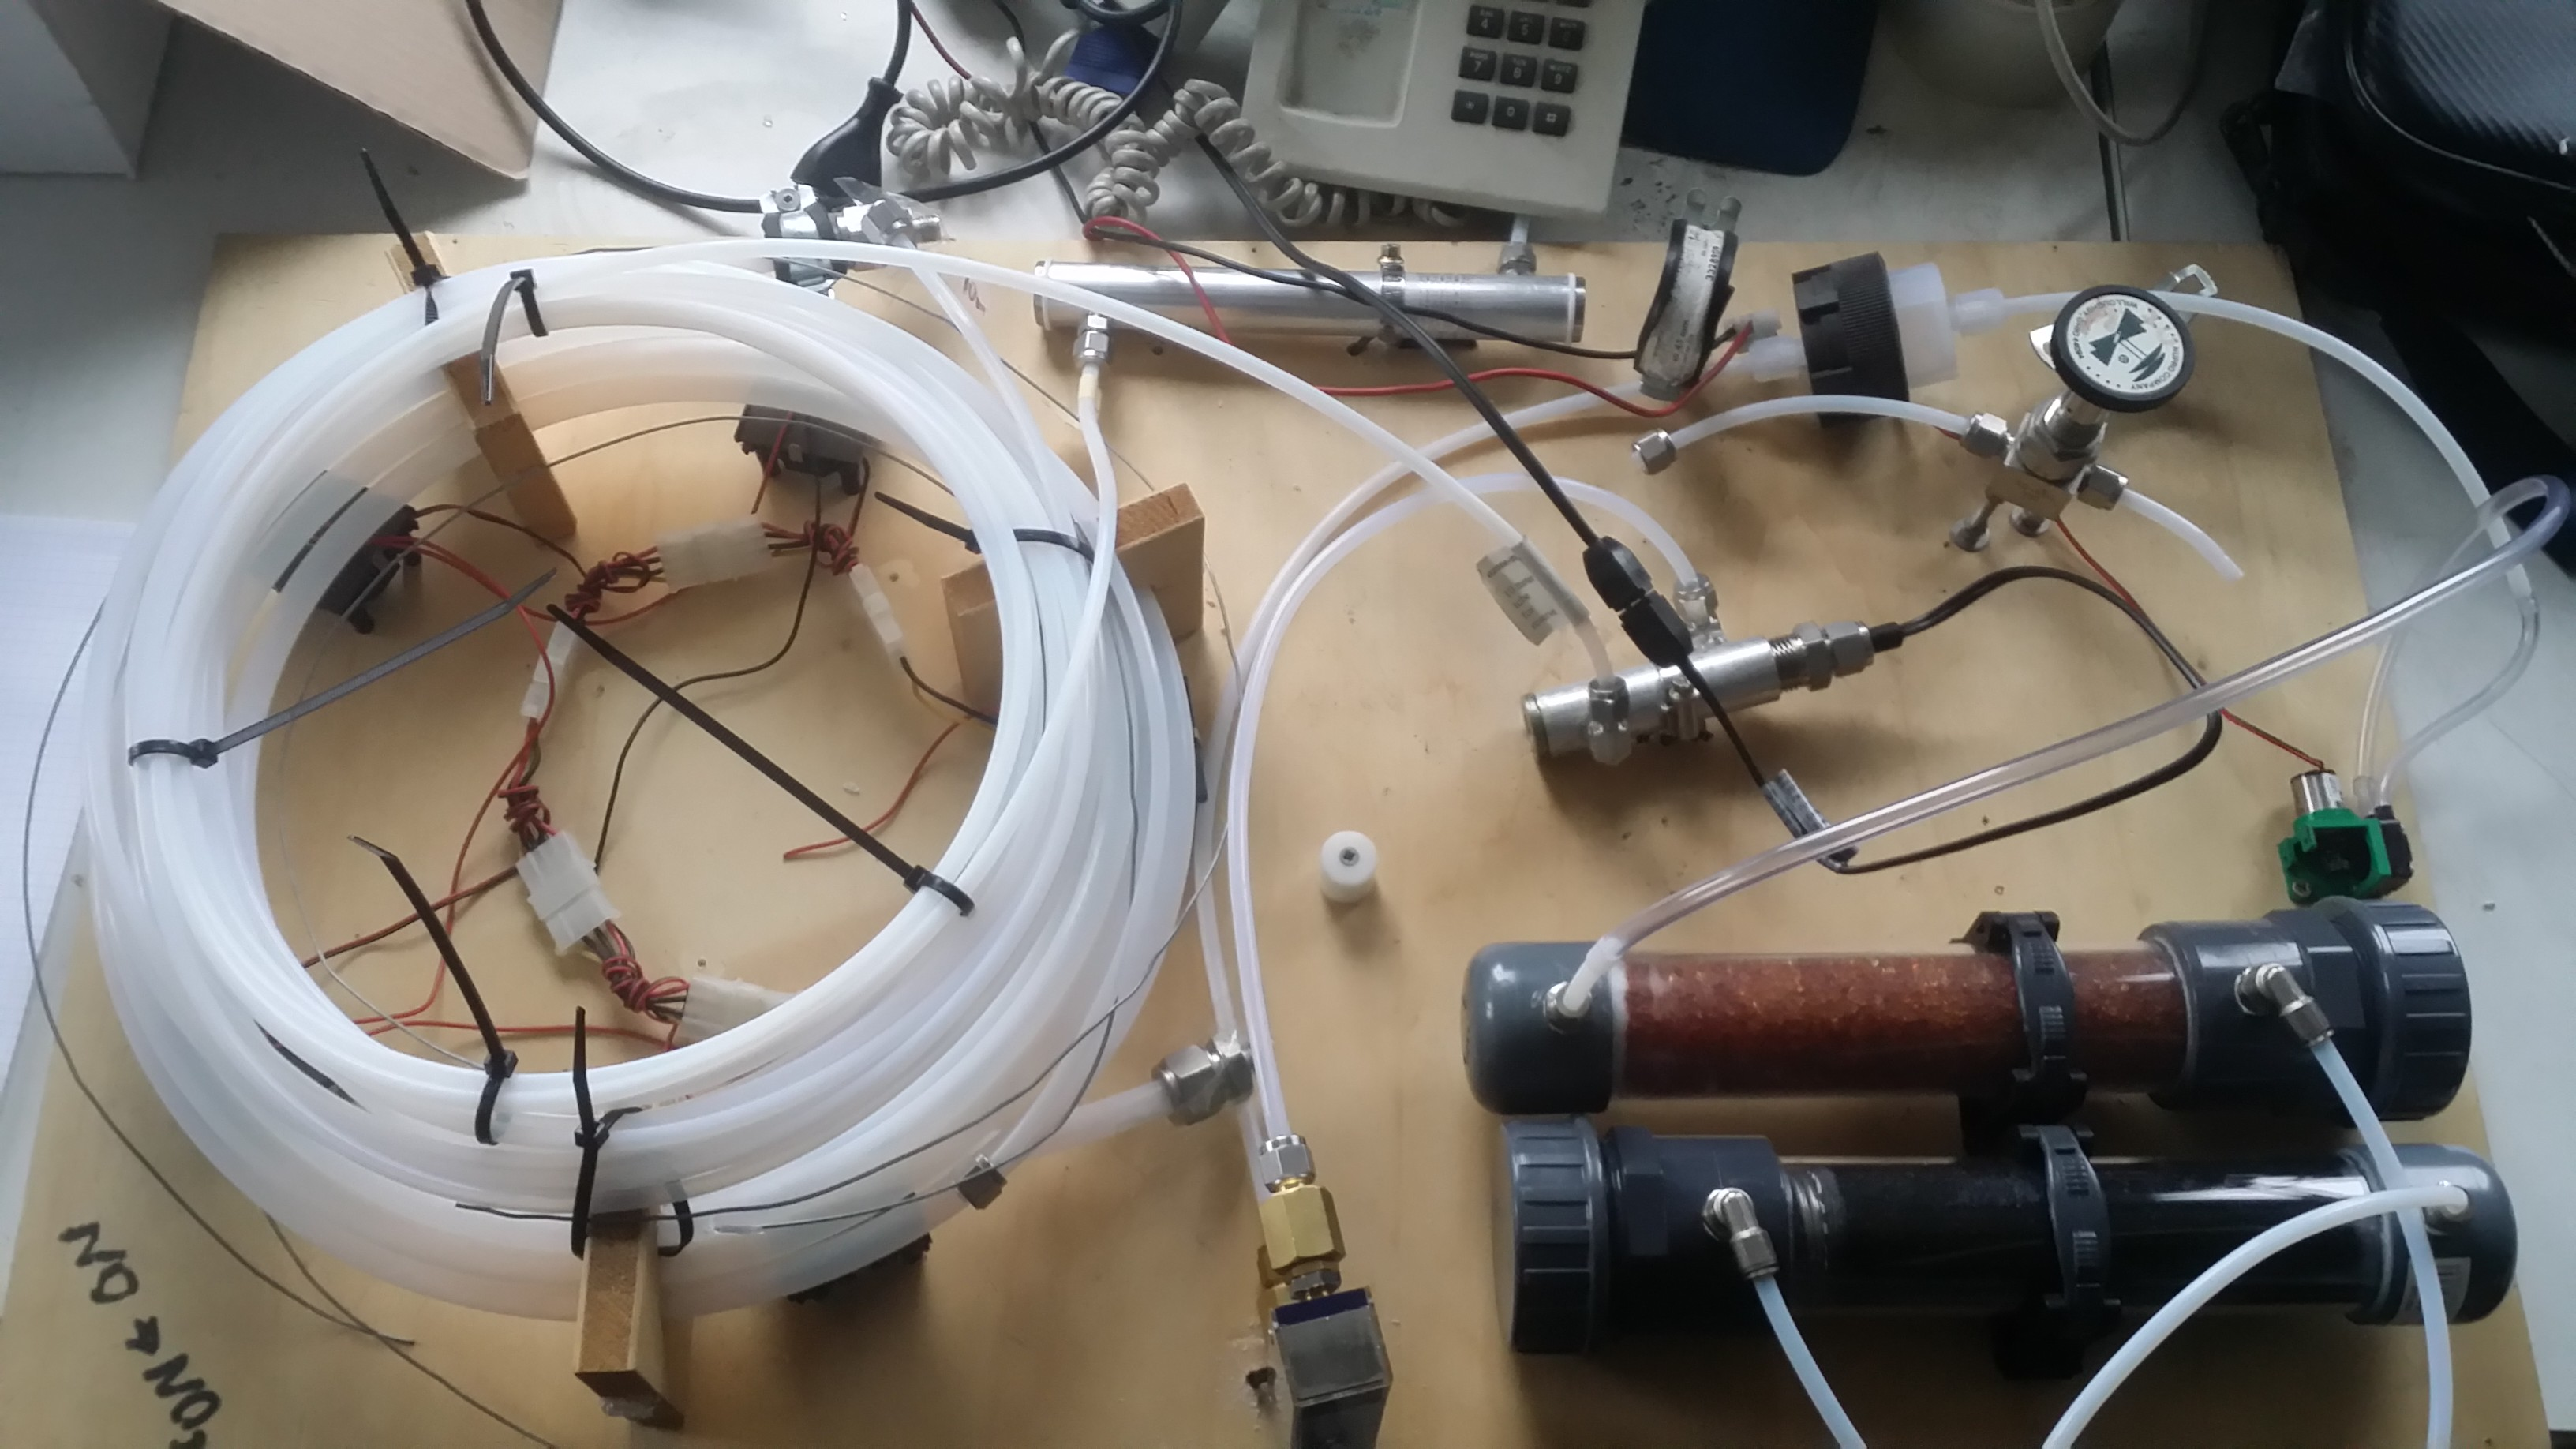
\includegraphics[width=0.9\linewidth]{setup.jpg}
  \caption{Ozone generator setup. Schematic and picture.}
  \label{fig:setup}
\end{figure}

The cuvette was entered into the ligthpath of a longpath DOAS
instrument (attached to an Amundsen telescope located at the height
laboratory at the IUP building). Since we expected rather high Ozone
concentrations, we forgo the advantage of a cavity enhanced
pathlength. The upside of this setup was that the instrument contained
a UV led emitting around a wavelength of $\lambda =
\SI{290}{\nano\meter}$. As mentioned in
Section~\ref{sec:theory-ozone}, Ozone has a strong absorption cross
section in this region, which allows us to determine the concentration
very precisely.\todo{ask Denis how to denote instrument}

\subsection{Inclusion into a CE-DOAS instrument}
\label{sec:inclusion}

\begin{figure}[htbp]
  \centering
  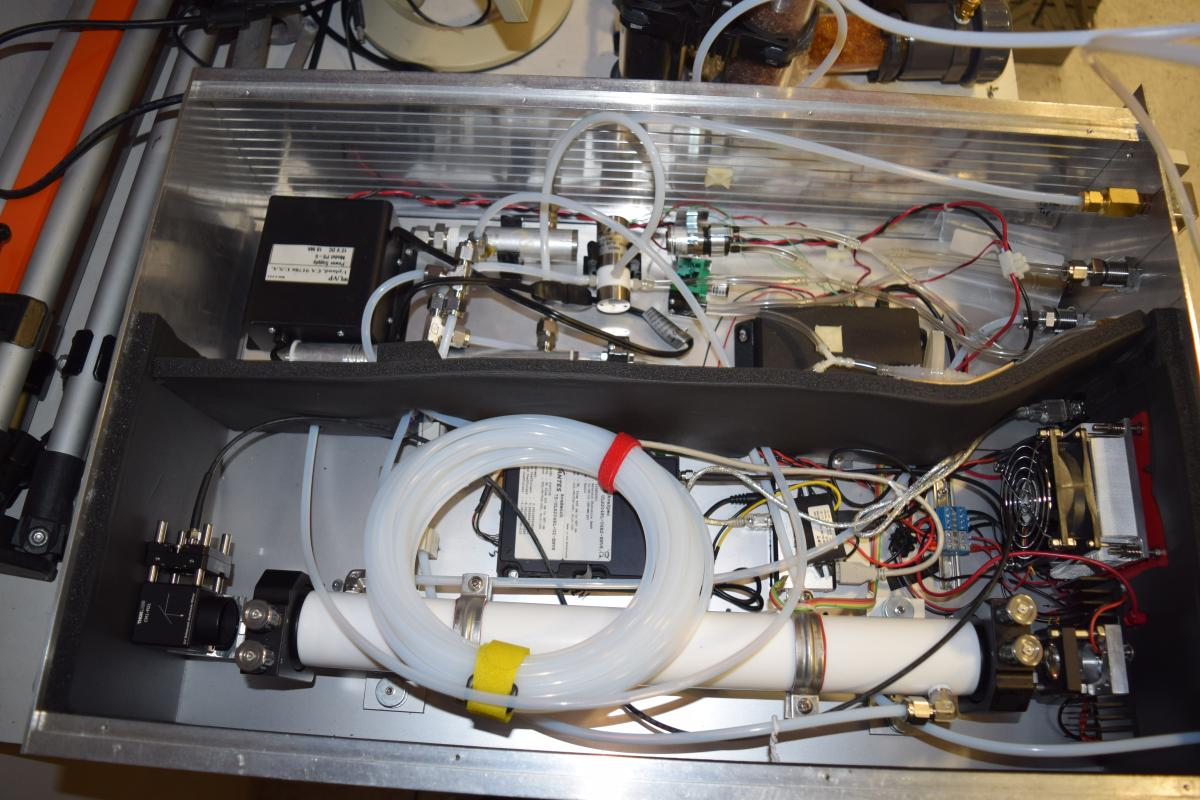
\includegraphics[width=0.8\textwidth]{images/envimes_up.jpg}
  \caption{EnviMeS CE-DOAS instrument with \ch{NO} to \ch{NO2}
    converter. On the upper left part the Pen-Ray lamp with
    powersupply can be seen. Below the powersupply partly covered by
    styrofoam is the additional Silica gel filter. In the lower half
    one can see the cavity with spectrometer and \SI{10}{\meter}
    reaction path rolled up.}
  \label{fig:envimes}
\end{figure}

\begin{figure}[htbp]
  \centering
  
\includegraphics[width=0.8\textwidth]{images/envimes_setup.png}
  \caption{Schematic of EnviMeS CE-DOAS instrument with \ch{NO} to
    \ch{NO2} converter.}
  \label{fig:envimes-schematic}
\end{figure}

After the above setup was tested the converter was added to an
existing CE-DOAS instrument (EnviMeS SN:2014002)\todo{technical data
  of envimes}. The instrument was already supplied with an \ch{O3}
generator, but lacked a Silica gel filter, which was added. The inside
of the instrument can be seen in Figure~\ref{fig:envimes}. Since it
was optimized for space, it is difficult, if not impossible, to extract
the setup from this view. Therefore Figure~\ref{fig:envimes-schematic}
contains a slightly simplified schematic view of the instrument. The
Zero Air input\todo{write zero air somewhere in theory} is used to
generate the Ozone, since it is already filtered. After the Hg-lamp
there is a \SI{1}{\meter} reaction path before the silica filter
follows. After that we have a Ozone bypass valve, which is operated
electromechanically and allows us to switch between an Ozone free and
an Ozone enriched air flow in the cavity. The sample air (with or
without Ozone) passes a \SI{10}{\meter} reaction path. In later
experiments the length of the reaction path was varied to measure the
influence on the \ch{NO} conversion (c.\,f.\
Sec.~\ref{sec:requirements} for the theory and Sec.~\ref{sec:no} for
measurements). The current for the Pen-Ray lamp was fixed. The total
flow $\Phi$ could be adapted, but was always set to
\SI{2}{\liter\per\minute}. The Ozone flow could be adapted (as in
Sec.~\ref{sec:ozone-setup}) from 0 to \SI{0.3}{\liter\per\minute}. The
lowest stable positive flow was \SI{0.03}{\liter\per\minute}. To
determine the Ozone production rate this flow was varied. When actual
\ch{NO} or \ch{NO_x}\todo{define NOx somewhere} measurements were
performed the flow was fixed to \SI{0.03}{\liter\per\minute}.

%%% Local Variables:
%%% mode: latex
%%% TeX-master: "../Bachelor"
%%% End:
